%% Elsevier elsarticle manuscript for Results in Engineering.
%% Template source: official Elsevier elsarticle bundle, downloaded from Elsevier.

\documentclass[preprint,12pt]{elsarticle}

\usepackage{amsmath}
\usepackage{amssymb}
\usepackage{booktabs}
\usepackage{graphicx}
\usepackage{multirow}
\usepackage{url}
\usepackage{xcolor}
\usepackage{lineno}
\usepackage{float}
\usepackage{placeins}

\makeatletter
\setlength{\@fptop}{0pt}
\setlength{\@fpsep}{14pt}
\setlength{\@fpbot}{0pt plus 1fil}
\makeatother
\renewcommand{\topfraction}{0.95}
\renewcommand{\bottomfraction}{0.95}
\renewcommand{\textfraction}{0.06}
\renewcommand{\floatpagefraction}{0.78}
\setlength{\textfloatsep}{14pt plus 3pt minus 3pt}
\setlength{\floatsep}{12pt plus 3pt minus 3pt}

\journal{Results in Engineering}

\biboptions{sort&compress}

\begin{document}

\begin{frontmatter}

\title{Risk- and reserve-aware receding-horizon planning for wind-affected UAV infrastructure inspection: a simulation study}

\author[inst1]{Haochen Li}
\author[inst1,inst2]{Junhao Wei}
\author[inst1]{Dexing Yao}
\author[inst1]{Yifu Zhao}
\author[inst1]{Yanxiao Li}
\author[inst1]{Zhaoyan Mai}
\author[inst1]{Jiamu Yu}
\author[inst1]{Baili Lu}
\author[inst3]{Sio-Kei Im}
\author[inst1]{Xu Yang}
\author[inst1]{Yapeng Wang\corref{cor1}}
\ead{yapengwang@mpu.edu.mo}
\cortext[cor1]{Corresponding author}
\affiliation[inst1]{organization={Faculty of Applied Sciences, Macao Polytechnic University},
            city={Macao},
            postcode={999078},
            country={China}}
\affiliation[inst2]{organization={Pazhou Lab (Huangpu)},
            city={Guangzhou},
            postcode={510555},
            country={China}}
\affiliation[inst3]{organization={Macao Polytechnic University},
            city={Macao},
            postcode={999078},
            country={China}}

\begin{abstract}
UAV infrastructure inspection exposes a planning conflict that standard coverage routing does not resolve: a vehicle must collect inspection value while wind-dependent energy use, obstacle clearance risk and return reserve remain feasible at the same time. Recent UAV planners already combine energy, wind, risk and online safety checks in several forms, so this paper does not claim a new planning paradigm. Instead, it studies an inspection-oriented receding-horizon implementation and introduces RR-CMP, a residual-margin packing step that uses only remaining feasible return, reserve and clearance margin to add targets. RAWA-RHP combines tail-aware wind budgeting, adaptive reserve, clearance-risk filtering, beam search and RR-CMP in one simulation planning layer. In paired simulation scenarios, RAWA-RHP improved safe weighted coverage over the strongest implemented baseline, FairALNSPlanner, by 0.1447 in blind scenarios and by 0.2019 under a gust multiplier of 3.0; both gains had positive 95\% confidence intervals and Holm-corrected significance. Formal ablations over 5760 full-mode episodes showed the largest fixed-pipeline contribution from RR-CMP, with smaller positive dependencies from adaptive search, risk control, adaptive reserve and beam search under native, equal-time and equal-evaluation budgets. A strict single-worker latency benchmark reported p95/p99 replanning latencies of 1.7549/1.7590 s with zero hard failures in the evaluated formal simulation checks. RAWA-RHP is a simulation-based planning layer, not hardware flight validation or low-level collision avoidance.
\end{abstract}

\begin{keyword}
UAV inspection \sep receding-horizon planning \sep wind-aware routing \sep risk-aware planning \sep safe weighted coverage \sep adaptive reserve \sep orienteering
\end{keyword}

\end{frontmatter}

%% \linenumbers

\section{Introduction}

Unmanned aerial vehicles (UAVs) are increasingly used to inspect infrastructure that is long, elevated, remote or hazardous for human inspectors. Power lines, transmission towers, wind turbines and bridges have motivated UAV-based inspection systems, imaging pipelines and route-planning studies \cite{Shakhatreh_2019,Khaloo_2017,Dorafshan_Maguire_2018,Dorafshan_2018,Kim_2018,Car_2020,Zhang_2024,Ahmed_2024,Yin_2022}. In these missions, the planner decides target value collection and safe return. It determines which assets are observed and when inspection must stop.

Wind, battery limits, obstacles and return reserve make infrastructure inspection different from ordinary coverage routing. Wind changes travel energy in a direction-dependent way, obstacles make high-value viewpoints risky, and a route that appears efficient can become unsafe if it spends the reserve needed for return. These effects are most pronounced around coastal transmission corridors, mountain power lines, wind farms, bridge decks and tower-like structures, where gusts, clutter and narrow passages interact with limited onboard energy.

Prior work has studied UAV routing under weather and energy constraints \cite{Thibbotuwawa_2019}, wind-aware path planning \cite{Thanellas_2019,Li_2024,Lian_2025,Gu_2026}, power-line inspection path optimisation \cite{Wu_2022,Li_AStar_2024}, human-UAV infrastructure inspection planning \cite{Pan_2024}, orienteering and route-improvement heuristics \cite{Vansteenwegen_2011,Ropke_2006,Mattos_Ribeiro_2012,Sacramento_2019}, and risk-aware or chance-constrained planning \cite{Blackmore_2011,Song_2018,Cai_2021,Nakka_2023,VeigaPineiro_2025,Qiu_2026}. Recent receding-horizon, wind-aware and risk-aware UAV studies already integrate several of these signals for online planning \cite{Ahmed_Sheltami_2024,Hu_2026,Gu_2026}. The remaining issue addressed here is narrower: after return, reserve and clearance checks have already constrained a route, how can the residual feasible margin be converted into additional inspection coverage without breaking those checks?

We address this narrower issue with RAWA-RHP, a Risk- and Reserve-Aware Wind-Adaptive Receding-Horizon Planner. Its implementation combines mature components: q90 energy-return budgeting, adaptive reserve, clearance-risk filtering, beam search and repair. The algorithmic emphasis is RR-CMP, a marginal packing post-processing step that inserts additional targets only when q90 return, reserve and clearance constraints remain satisfied. At each replan step, the planner updates state and scenario context, builds candidate route prefixes, applies those checks, executes the first action and replans.

The contributions are fivefold. First, we formulate safe weighted coverage (SWC) as a benchmark metric for wind-affected UAV infrastructure inspection. Second, we introduce RR-CMP as a residual-margin target-packing rule within a receding-horizon inspection planner. Third, we provide paired baseline comparisons against greedy, reserve-only, risk-aware greedy and FairALNSPlanner baselines. Fourth, we report equal-budget ablations that separate RR-CMP and other fixed-pipeline dependencies from extra computation. Fifth, we evaluate strict replanning latency and hard-failure outcomes in the proposed benchmark. The contribution is therefore an inspection-specific planning-layer implementation and RR-CMP post-processing rule, not a claim that rolling horizon planning, quantile energy budgets, risk filtering or beam search are new planning paradigms.

\section{Related work}

\subsection{UAV inspection of risk-critical infrastructure}

UAV inspection has been studied for civil infrastructure, bridge modelling, crack detection, wind-turbine blade inspection and power-line inspection \cite{Shakhatreh_2019,Khaloo_2017,Dorafshan_Maguire_2018,Dorafshan_2018,Kim_2018,Car_2020,Zhang_2024,Ahmed_2024,Yin_2022}. Much of this literature focuses on sensing, reconstruction or defect detection, while route planning is often treated as a supporting component. Bridge and wind-turbine studies show the value of close-range UAV acquisition, but they also expose the operational difficulty of maintaining clearance around large structures \cite{Khaloo_2017,Car_2020,Zhang_2024}. Power-line and transmission-tower studies add the challenge of elongated assets, repeated inspection targets and wind exposure \cite{Ahmed_2024,Wu_2022,Li_AStar_2024,Li_2024}.

The present work treats these inspection domains as instances of one planning problem: a UAV must collect value from spatially distributed targets while preserving energy and clearance margin. The proposed benchmark abstracts the asset type, but keeps the constraints that make these missions difficult: wind-dependent energy, obstacle density, narrow passages, correlated gusts and safe return.

\subsection{Coverage, orienteering and adaptive route search}

Inspection routing is closely related to the orienteering problem, where a path collects rewards under a travel budget \cite{Vansteenwegen_2011}. Team orienteering and time-window variants have motivated local-search and iterated-search heuristics \cite{Vansteenwegen_2009}. Adaptive large neighbourhood search (ALNS) is a strong family of routing heuristics and has been applied to pickup-and-delivery, vehicle routing and drone-assisted routing problems \cite{Ropke_2006,Mattos_Ribeiro_2012,Sacramento_2019}. These methods are effective for improving routes under combinatorial constraints, and they motivate FairALNSPlanner as the strongest implemented baseline in this study.

RAWA-RHP differs from offline route improvement in two ways. First, it replans in a receding-horizon loop, so it can update decisions as the state and remaining reserve change. Second, it treats the travel budget as risk- and wind-dependent rather than fixed. The marginal packing component is inspired by route improvement, but it is only accepted when the remaining energy and clearance-risk margins support the insertion.

\subsection{Wind-aware, risk-aware and receding-horizon planning}

Wind-aware planning has been studied for UAV routing under weather forecasts, spatial wind fields and energy consumption constraints \cite{Thanellas_2019,Thibbotuwawa_2019,Lin_2024,Lian_2025,Gu_2026}. Recent studies also integrate wind-field analysis with safety and energy efficiency, use CFD or learned wind surrogates for risk-aware planning, and address energy-aware coverage in difficult terrain \cite{Gu_2026,VeigaPineiro_2025,Shao_2025}. Risk-aware and chance-constrained planning provide related tools for dealing with uncertainty and obstacles \cite{Blackmore_2011,Song_2018,Cai_2021,Nakka_2023}. Receding-horizon planning and real-time MPC variants are also relevant when the planner must repeatedly trade computational cost against updated state information \cite{Mandalika_2018,Ahmed_Sheltami_2024,Hu_2026,Qiu_2026}.

These works mean that the present paper should not be read as claiming the first integration of risk, energy and online UAV planning. RAWA-RHP is designed as an operational inspection planner that combines established components under one benchmark. Its specific algorithmic addition is RR-CMP: after the receding-horizon planner has produced a feasible prefix, RR-CMP searches for target insertions that consume only residual return, reserve and clearance margin. The question tested here is therefore whether that residual-margin packing rule and the fixed planning pipeline improve SWC under paired, equal-budget simulation checks.

\section{Problem formulation}

We consider a UAV inspection episode specified by a depot, a finite set of inspection targets, non-negative target values, a wind profile and wind level, an obstacle-density setting, the initial battery state and evaluated simulation check thresholds. The wind profile determines direction-dependent travel energy. The obstacle setting determines the clearance-risk context. The target values define the reward that can be collected before the UAV must return to the depot.

At each replan step, the planner observes a state containing the current node, remaining battery, visited and unvisited targets, the current scenario context and the constraints used for feasibility checks. The action is the next route decision: either move toward the first target of the selected route prefix or return when the planning loop judges that further inspection is not feasible under the energy and reserve envelope. The planner therefore solves a repeated local decision problem rather than a one-shot offline tour.

The objective is to maximise safe weighted coverage. Let $V$ be the total value of all targets and let $V_{\mathrm{visited}}$ be the value collected in an episode. The weighted coverage is
\begin{equation}
    C = \frac{V_{\mathrm{visited}}}{V}.
\end{equation}
The safe weighted coverage is
\begin{equation}
    C_{\mathrm{safe}} =
    \begin{cases}
    C, & \text{if no evaluated hard failure occurs},\\
    0, & \text{otherwise,}
    \end{cases}
\end{equation}
where evaluated hard failure includes battery violation, clearance violation, reserve shortfall, return failure and emergency abort in the proposed benchmark. This definition intentionally penalises routes that obtain high coverage by consuming infeasible margins.

Unsafe high-coverage routes receive zero SWC because they do not satisfy the benchmark goal of inspection: target observations are counted only if the vehicle avoids the hard failures measured in this study. The term ``hard failure'' is limited to the evaluated simulation hard-failure checks: battery violation, clearance violation, reserve shortfall, return failure and emergency abort. It is not a claim about real-world flight outcomes outside the simulated planning layer.

\begin{table}[!htbp]
\centering
\caption{Hard failure definitions used by the evaluated simulation hard-failure checks.}
\label{tab:failure-definitions}
\resizebox{\textwidth}{!}{%
\begin{tabular}{lp{0.72\textwidth}}
\hline
Failure type & Definition in the simulator \\
\hline
Battery violation & Remaining battery becomes negative during an inspection leg or the final return leg. \\
Clearance violation & Expected clearance-event rate exceeds 0.05, or the minimum path clearance is below UAV radius plus clearance buffer ($0.35 + 0.80$). \\
Reserve shortfall & Final battery minus the reserve floor is negative; the reserve floor is 80 energy units. \\
Return failure & The vehicle cannot complete the planned return with non-negative battery. \\
Emergency abort & A battery violation occurs during execution, triggering an immediate abort flag. \\
\hline
\end{tabular}
}
\end{table}


Reserve shortfall in Table~\ref{tab:failure-definitions} is a benchmark-level hard-failure check based on the fixed reserve floor $F=80$. The adaptive reserve in Eq.~\eqref{eq:adaptive-reserve} is a planner-level feasibility and ranking rule used by RAWA-RHP during decision making. These two reserve quantities have different roles: one defines the benchmark failure event, while the other controls route construction.

The planner is evaluated under paired scenarios so that different algorithms face the same map, wind profile and level, obstacle density, target set, battery setting, evaluated simulation check thresholds and stochastic seed. This pairing is important because SWC varies strongly with wind, geometry and target layout.

\section{Method}

\subsection{Overview}

RAWA-RHP is a receding-horizon planner for reward collection under wind, battery and clearance-risk constraints. Figure~\ref{fig:method} summarises the decision loop. Rolling horizon planning, quantile energy budgeting, risk filtering and beam search are established components. The distinct post-processing step in this implementation is RR-CMP, which tries to add targets only with residual feasible margin. The planner takes the current vehicle state, scenario context, target set and evaluated simulation check thresholds as input. It outputs the first executable action of a route prefix whose travel, return, reserve and clearance-risk checks remain feasible. It then replans after execution rather than committing to the entire route.

\begin{figure}[!htbp]
    \centering
    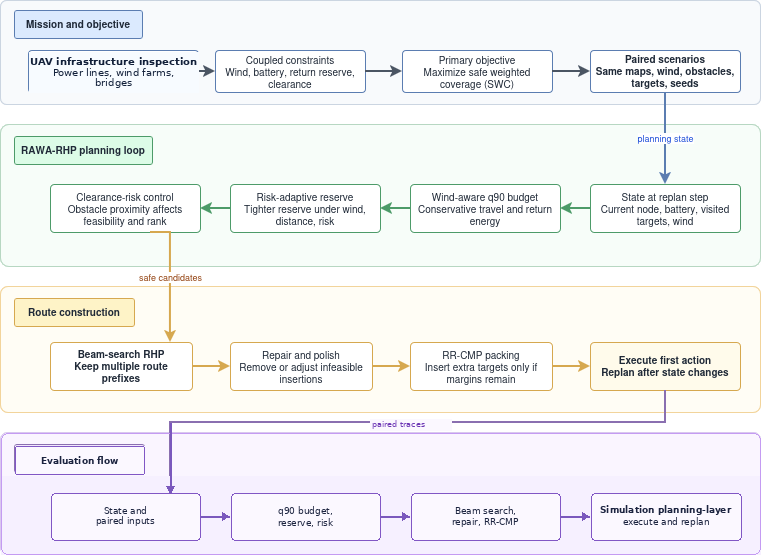
\includegraphics[width=\textwidth]{figures/rawa.png}
    \caption{RAWA-RHP planning loop. The simulation planning-layer flow is state update, q90 budget/reserve/risk estimation, beam search, repair and RR-CMP, then first-action execution and replanning.}
    \label{fig:method}
\end{figure}

\begin{table}[!htbp]
\centering
\caption{RAWA-RHP replanning pseudocode.}
\label{tab:rawa-pseudocode}
\resizebox{\textwidth}{!}{%
\begin{tabular}{p{0.97\textwidth}}
\hline
\textbf{Input:} current node $i$, unvisited targets $U$, remaining battery $b$, target values $v_j$, depot $0$, edge cache with distance, q90 energy and clearance-risk estimates, reserve and search-budget parameters. \\
\textbf{Output:} next node to execute, or return/stop if no candidate prefix is feasible. \\
\hline
1. Initialise beam with the empty prefix $((), i, 0, 0, 0, 0)$, where the tuple stores route, cursor, travel budget, value, accumulated risk and maximum edge risk. \\
2. For depth $d=1,\ldots,D$: build a candidate pool from $U$ using value-per-budget, return-aware value, low-risk and short-distance ranking keys. \\
3. For each beam state and candidate target $j$: compute leg budget $B_{ij}$, return budget $R_j$, route risk statistics and adaptive reserve $A(b,R_j,r)$. Reject the extension if $b-[T+B_{ij}+R_j] < A(b,R_j,r)$. \\
4. Add feasible extensions to the next beam. Remove dominated states with no higher value, lower cost or lower risk. Sort by the plan score in Eq.~\eqref{eq:plan-score}, keep at most $W$ states, and stop if the time or expansion budget is reached. \\
5. Repair top prefixes by insertion/local polish. A repair move is kept only if the updated prefix passes the same battery-return-reserve check and the configured risk-control rule. \\
6. Run RR-CMP. For each remaining target and insertion position, compute marginal value, marginal q90 budget and marginal clearance risk. Accept the best positive-gain insertion only if $b-[T'+R'] \ge A(b,R',r')$ and the configured clearance-risk control remains satisfied. Repeat until no positive insertion, no candidate, or the insertion/time budget is exhausted. \\
7. Return the first target of the best feasible prefix; if no prefix remains, return/stop. Execute the first action and replan after the simulator updates the state. \\
\hline
\end{tabular}
}
\end{table}

\subsection{State update and candidate pool}

This stage takes the current node, remaining battery, unvisited targets and edge cache as input; it decides which one-step target extensions are feasible; it outputs a ranked candidate pool for prefix expansion. At replan step $t$, the implementation receives current node $i_t$, unvisited targets $U_t$, remaining battery $b_t$, target values $v_j$ and the precomputed edge cache. For every candidate $j\in U_t$, the planner first computes a leg budget $B_{ij}$, a return budget $R_j$ and a return delta $\Delta R_j=\max(0,R_j-R_i)$. The candidate is rejected before ranking if
\begin{equation}
    b_t - \left(T_t + B_{ij} + e_{\mathrm{photo}} + R_j\right) < A(b_t,R_j,r_{ij}),
    \label{eq:single-feasibility}
\end{equation}
where $T_t$ is the prefix travel budget already committed inside the candidate prefix, $e_{\mathrm{photo}}=5.0$, $r_{ij}$ is the clearance-risk score of the leg and $A(\cdot)$ is the adaptive reserve in Eq.~\eqref{eq:adaptive-reserve}. Feasible candidates are ranked by a union of keys: $v_j/B_{ij}$, $v_j/(B_{ij}+0.35\Delta R_j)$, adaptive value per return-and-risk-adjusted budget, low detour, low return risk and high value. The selected pool is capped by the adaptive candidate-pool size in Table~\ref{tab:method-parameters}. If the pool is empty, the planner returns rather than forcing an inspection move.

\subsection{Wind-aware q90 travel and return budgeting}

This stage takes segment geometry and wind samples as input; it decides the q90 travel and return budgets; it outputs $B_{ij}$ and the return budget used in feasibility checks. For an edge path with segment lengths $\ell_s$, unit travel directions $d_s$ and wind samples $w_s$, the simulator computes
\begin{equation}
    \begin{aligned}
    E(w)&=\sum_s \ell_s\left(c_0+c_1 a_s^2+c_2 h_s^2\right)+c_{\mathrm{turn}}\Theta,\\
    a_s&=\min(\|v_{\mathrm{ground}}d_s-w_s\|,v_{\mathrm{air,max}}),\\
    h_s&=\max(0,-w_s^\top d_s),
    \end{aligned}
    \label{eq:energy-model}
\end{equation}
where $\Theta$ is the summed turn angle. Lengths and clearances are simulator distance units, wind and speed are distance units per second, and $E(w)$ is expressed in simulator energy units. The reported configuration uses $v_{\mathrm{ground}}=5.0$, $v_{\mathrm{air,max}}=12.0$, $c_0=1.0$, $c_1=0.045$, $c_2=0.070$ and $c_{\mathrm{turn}}=2.0$. Each edge stores the nominal estimate plus 32 gust samples. The q90 budget is the 0.90 quantile of these values. RAWA-RHP uses the adaptive energy variant in which the wind-induced increment relative to no-wind energy is reduced to 20\% when adverse and 92\% when favourable; the candidate budget then blends the adaptive mean toward the adaptive q90 statistic:
\begin{equation}
    B_{ij}=\bar{E}^{\mathrm{ad}}_{ij}+\lambda_{ij}\left(Q^{\mathrm{ad}}_{0.90,ij}-\bar{E}^{\mathrm{ad}}_{ij}\right).
    \label{eq:q90-budget}
\end{equation}
The blend $\lambda_{ij}$ is higher for return legs, high risk, high tail spread and low battery. Return feasibility uses the same budget on the edge from candidate endpoint to the depot.

\subsection{Adaptive reserve and clearance-risk control}

This stage takes segment clearance, cross-wind and battery-return pressure as input; it decides the path risk and planner-level reserve; it outputs $r_{\mathrm{path}}$ and $A(b,R,r)$. Clearance risk is computed from segment midpoints. Let $c_s$ be clearance, $m_s=c_s-r_{\mathrm{uav}}-b_{\mathrm{safe}}$ be clearance margin, $g_s$ be gust standard deviation and $q_s$ be the cross-wind magnitude. The implementation uses
\begin{equation}
    \sigma_s=\sigma_0+k_{\mathrm{cross}}q_s+k_{\mathrm{gust}}g_s,\qquad
    p_s=\Phi_{\mathrm{surv}}\left(\frac{m_s}{\max(\sigma_s,10^{-6})}\right),
    \label{eq:local-risk}
\end{equation}
then scales $p_s$ by segment length to obtain $\tilde{p}_s$. The path no-event probability is the product of segment no-event probabilities, giving
\begin{equation}
    P_{\mathrm{no\ event}}=\prod_s(1-\tilde{p}_s),\qquad
    r_{\mathrm{path}}=1-\prod_s(1-\tilde{p}_s).
    \label{eq:path-risk}
\end{equation}
The reserve rule converts battery pressure, return pressure and risk pressure into an energy reserve:
\begin{equation}
    \begin{aligned}
    A(b,R,r)=\max\big(&0.55F,\,
    F+\eta(0.28+0.26\rho_b+0.20\rho_R+0.26\rho_r)\\
    &+22\rho_b+18\rho_R+12\rho_r\big),
    \end{aligned}
    \label{eq:adaptive-reserve}
\end{equation}
where $F=80$ is the reserve floor, $\eta=16$ is the reserve buffer, $\rho_b=\max(0,1-b/E_{\max})$, $\rho_R=\min(1,R/E_{\max})$ and $\rho_r=\min(1,r/r_{\mathrm{avg}})$ with $r_{\mathrm{avg}}=0.075$. In the final RAWA-RHP configuration, clearance risk affects candidate ranking, reserve pressure and RR-CMP pricing. The evaluated simulation clearance failure is measured separately by the benchmark definition in Table~\ref{tab:failure-definitions}. Thus, $F=80$ is both the benchmark reserve floor for the hard-failure check and the base term from which RAWA-RHP constructs its adaptive planner-level reserve.

\subsection{Beam-search route-prefix expansion}

This stage takes the ranked candidate pool and current prefix states as input; it decides which feasible prefixes survive pruning; it outputs a beam of route-prefix candidates. Beam search stores route prefix $\pi$, cursor node, accumulated travel budget $T(\pi)$, collected value $V(\pi)$, accumulated risk and maximum edge risk. After each expansion, dominated states with no better value, cost or risk are removed. Remaining states are scored by
\begin{equation}
    S(\pi)=V(\pi)+0.05|\pi|+0.15\,u(b,T,R,A)-0.006\,C(\pi),
    \label{eq:plan-score}
\end{equation}
where $C(\pi)=T(\pi)+R_{\mathrm{last}(\pi)}$, and $u(\cdot)$ is a bounded reserve-utilisation term derived from the slack after adaptive reserve. The final configuration sets the explicit additive risk penalty to zero; risk enters through filtering and ranking, reserve pressure and RR-CMP pricing rather than an additional score term. The beam keeps at most $W$ prefixes until depth $D$, the expansion limit or the 1.75 s replanning budget is reached.

\subsection{Repair and RR-CMP marginal packing}

This stage takes the best feasible prefixes and remaining targets as input; it decides whether repair or marginal packing improves value without breaking feasibility; it outputs the final prefix used for execution. Repair evaluates insertion and local-polish moves on the best prefixes. For inserting target $j$ at position $k$, the implementation computes the change in total budget $\Delta C$, travel budget $\Delta T$, risk sum $\Delta r$ and maximum edge risk by replacing the affected edge or return edge. A repaired prefix is kept only if
\begin{equation}
    b-\left[C(\pi)+\Delta C\right]\ge A\left(b,R'_{\pi},r'_{\pi}\right).
    \label{eq:repair-accept}
\end{equation}
RR-CMP then uses the same marginal calculation to insert additional targets into a feasible prefix. It computes energy and risk shadow prices from reserve pressure and risk pressure, and accepts the candidate with the largest positive gain
\begin{equation}
    G_j=v_j+B_{\mathrm{regret}}+B_{\mathrm{slack}}
    -\lambda_E\max(0,\Delta C)-\lambda_R\max(0,\Delta r),
    \label{eq:packing-gain}
\end{equation}
subject to Eq.~\eqref{eq:repair-accept}. Insertions stop when no candidate has positive gain, no candidates remain, the insertion limit is reached or the time budget is exhausted. This rule is why RR-CMP can increase coverage without accepting a target that breaks the q90 return and adaptive-reserve envelope used by the planner.

\subsection{Adaptive search budget and receding-horizon execution}

This stage takes scene-level risk, tail-energy spread and remaining-task pressure as input; it decides the search budget and first executable action; it outputs one action before the next replan. The search controller computes scene-level risk summaries and tail-energy spread from the edge cache. Low-risk scenes use smaller budgets; high-risk or high-opportunity scenes increase beam width, candidate pool size, repair depth, packing candidates and expansion limits. During a replan, the budget is further adjusted by remaining-target pressure, battery pressure and environmental risk pressure. Only the first target of the selected prefix is executed. The simulator then samples actual edge energy, updates battery and state, and calls the planner again. Equal-time and equal-evaluation ablations calibrate this component so that the reported gains are not explained only by extra computation.

\subsection{Parameter selection and calibration}

The reported parameter values are fixed configuration choices used consistently across all reported experiments, not per-scenario tuning. The q90 energy statistic was selected to give a tail-aware return budget without making every edge follow a more conservative q95 rule. Each edge stores the nominal wind estimate plus 32 gust samples so that the tail budget is estimated from repeated gust realisations while keeping the edge cache small enough for repeated replanning.

The reserve floor $F=80$ is the benchmark-level reserve floor used in the hard-failure checks. The reserve buffer $\eta=16$ and pressure weights in Eq.~\eqref{eq:adaptive-reserve} are fixed planner settings that determine how battery pressure, return pressure and clearance-risk pressure raise the planner-level reserve above that floor. The clearance buffer of 0.80 and clearance-event threshold of 0.05 are simulation benchmark thresholds. Beam width, horizon length, candidate-pool size, repair limits, RR-CMP limits, expansion limits and the 1.75 s replan cap were fixed before the reported comparisons and then used consistently across blind, gust-stress and formal ablation experiments. Implementation details and configuration files should be reported in the supplementary archive or code release.

\subsection{Simulation model parameterisation and validity checks}

The simulator is a parameterised planning-layer model, not a hardware-calibrated flight-energy or collision-probability model. We therefore check model plausibility rather than claiming real-flight calibration. The energy sanity check varies headwind, tailwind and crosswind components on a fixed segment and verifies non-negative energy, increasing cost under adverse wind and bounded tailwind benefit after the adaptive-energy transform. The clearance-risk sanity check varies clearance margin, crosswind and gust standard deviation and verifies that event probability decreases with increasing margin and increases under wind/gust dispersion. The scenario-validity check documents how ID, severe-wind, correlated-gust, narrow-passage and gust-stress profiles cover low-risk, nominal, pressure and OOD planning-layer conditions. Full curves and source data are provided in the reproduction package.

\subsection{Parameter sensitivity protocol}

We ran an additional one-factor-at-a-time sensitivity subset to check whether the final parameters form a broad operating region rather than a seed-specific optimum. The subset used seeds 301--307 across the same three profiles, three wind levels and two obstacle densities, giving 126 paired scenarios. Each variant changed one parameter family while keeping the final pipeline fixed: energy quantile, reserve floor, reserve buffer, clearance threshold, risk dispersion scale, beam/search budget, horizon length, RR-CMP weights, gust-sample count or replan cap. The reported statistic is $\Delta$SWC, variant minus final setting, on the same paired scenario. This subset is not used to replace the formal baseline or ablation evidence.

\begin{table}[!htbp]
\centering
\caption{RAWA-RHP implementation parameters used in the reported experiments. Adaptive ranges are produced by the risk- and opportunity-dependent search-budget rule.}
\label{tab:method-parameters}
\resizebox{\textwidth}{!}{%
\begin{tabular}{llll}
\hline
Parameter group & Value & Role & Selection note \\
\hline
Beam width & Initial 96; adaptive 240--560 & Number of route prefixes retained after pruning. & Fixed search configuration. \\
Horizon length & Initial 7; adaptive 10--12 & Maximum prefix depth expanded within one replanning step. & Fixed receding-horizon range. \\
Candidate pool size & Initial 16; adaptive 34--72 & Maximum target candidates retained for expansion. & Fixed candidate-generation range. \\
Repair candidates & top-$k$ 18--56; insertions 22--48 & Number of prefixes and insertions considered during repair. & Fixed repair range. \\
RR-CMP candidates & Initial 18; adaptive 18--48 & Maximum marginal-packing candidates per repair pass. & Fixed marginal-packing range. \\
Energy quantile & q90 & Tail statistic for travel and return energy budgeting. & Tail-budget setting used consistently. \\
Gust samples & 32 plus nominal estimate & Edge-level samples used for tail-budget estimation. & Fixed sampling count for the edge cache. \\
Energy model & $c_0=1.0$, $c_1=0.045$, $c_2=0.070$, $c_{\mathrm{turn}}=2.0$ & Per-metre and turning-energy coefficients. & Simulator configuration. \\
Reserve parameters & floor 80; buffer 16; pressure weights 22/18/12 & Minimum reserve plus battery, return and risk-pressure terms. & Benchmark floor plus fixed adaptive range. \\
Risk parameters & $\sigma_0=0.25$, $k_{\mathrm{cross}}=0.08$, $k_{\mathrm{gust}}=0.05$, $p_{\max}=0.08$ & Clearance-risk dispersion and reference cap. & Fixed clearance-risk model configuration. \\
Simulation check thresholds & clearance buffer 0.80; event threshold 0.05 & Thresholds used by benchmark hard-failure checks. & Benchmark thresholds. \\
Risk/pricing weights & insertion 18; packing regret 0.38; packing unlock 0.24 & Penalties and bonuses used in insertion and RR-CMP scoring. & Fixed route-packing configuration. \\
Search budget & 1.75 s; adaptive 30k--86k expansions & Runtime and expansion termination limits per replan. & Fixed runtime and expansion cap. \\
Termination & no feasible target, all targets visited, expansion/time budget, or battery abort & Conditions that end a replan or episode. & Fixed stopping conditions. \\
\hline
\end{tabular}
}
\end{table}


\FloatBarrier

\section{Experimental setup}

\subsection{Scenarios and algorithms}

The main comparison evaluates RAWA-RHP against simple greedy planners, a wind-aware greedy planner, ReserveOnlyPlanner, FairRiskAwareGreedy and FairALNSPlanner. Scenarios are paired across planners: the map, wind profile and level, obstacle density, target set, battery setting, evaluated simulation check thresholds and stochastic seed are fixed within each paired comparison. This design makes the reported differences planner differences rather than differences in geometry or wind realisation.

FairALNSPlanner is treated as the strongest implemented baseline in this configuration because adaptive large-neighbourhood search is a strong route-improvement family for reward-collecting routing problems. It can revise route structure more extensively than greedy, reserve-only or single-step risk-aware rules, so it is the most demanding implemented comparator in the final paired statistics. This does not claim that the baseline set exhausts all possible planners. The blind suite does not give planners favourable scenario-specific tuning. It evaluates the configured planners on shared scenarios rather than adapting parameters to individual wind or obstacle cases.

Two main scenario families are reported. The blind scenario suite contains 600 paired episodes and covers wind levels, obstacle densities and target sets. The gust-stress suite contains 400 paired episodes with an actual gust multiplier of 3.0. Both suites compare algorithms on the same paired seeds.

Formal ablations use a full-mode matrix with 20 seeds, three scenario profiles (in-distribution, correlated gust and narrow passage), three wind levels (calm, moderate and severe) and two obstacle densities (sparse and cluttered). This gives 360 shared scenarios. The formal ablation run contains 5760 episodes: RAWA-RHP plus five core modules under three budget regimes.

\begin{table}[!htbp]
\centering
\caption{Scenario configuration used by the reported experiments.}
\label{tab:scenario-config}
\resizebox{\textwidth}{!}{%
\begin{tabular}{llll}
\hline
Item & Blind suite & Gust-stress suite & Formal ablation suite \\
\hline
Episodes & 600 paired episodes & 400 paired episodes & 5760 episodes over 360 shared scenarios \\
Seeds and profiles & Shared seeds; in-distribution profile & Shared seeds; in-distribution profile & seeds 1--20; ID, correlated gust, narrow passage \\
Wind levels & calm, moderate, severe & moderate, severe & calm, moderate, severe \\
Gust multiplier & 1.0 & 3.0 applied to sampled-energy deviation from mean & 1.0 \\
Obstacle density & sparse and cluttered & sparse and cluttered & sparse and cluttered \\
World and grid & 100 by 100 world; 50 by 50 grid & same & same \\
Depot & fixed at $(8,8)$ for reported profiles & fixed at $(8,8)$ & fixed at $(8,8)$ \\
Targets & 32 targets; values $\{1,1.5,2,2.5,3\}$ with probabilities $\{0.16,0.20,0.28,0.20,0.16\}$ & same & same \\
Obstacle generation & 7 sparse or 13 cluttered rectangles; targets sampled near obstacles with probability 0.78 & same & same, with additional narrow-passage bars for that OOD profile \\
Wind bands & calm 0.6--1.8, moderate 3.0--5.0, severe 6.0--8.0; gust bases 0.35/0.75/1.20 & same bands; execution multiplier 3.0 & same bands; correlated-gust profile shares gust components \\
\hline
\end{tabular}
}
\end{table}

\begin{table}[!htbp]
\centering
\caption{Vehicle, energy and hard-failure check parameters used by the simulator.}
\label{tab:vehicle-check-config}
\resizebox{\textwidth}{!}{%
\begin{tabular}{lll}
\hline
Parameter group & Value & Role in the evaluated simulation benchmark \\
\hline
Battery and speed & battery 1200; ground speed 5.0; max air speed 12.0 & Vehicle energy envelope and velocity limits. \\
Inspection cost & photo energy 5.0; photo time 2.0 & Per-target observation cost. \\
Energy coefficients & $c_0=1.0$, $c_1=0.045$, $c_2=0.070$, $c_{\mathrm{turn}}=2.0$ & Wind-dependent travel and turning energy. \\
Reserve check & fixed reserve floor 80 & Benchmark-level reserve-shortfall threshold. \\
Clearance check & UAV radius 0.35; clearance buffer 0.80; event threshold 0.05 & Clearance hard-failure check thresholds. \\
Risk dispersion & $\sigma_0=0.25$, $k_{\mathrm{cross}}=0.08$, $k_{\mathrm{gust}}=0.05$ & Segment-level clearance-event model. \\
Episode termination & all targets visited, no feasible next target, return completion, battery violation, or emergency abort & Simulator stopping conditions. \\
\hline
\end{tabular}
}
\end{table}


\FloatBarrier

\subsection{Planner information access}

The baselines differ in the information and checks they are allowed to use (Table~\ref{tab:planner-settings}). ReserveOnlyPlanner uses wind-aware tail budgets, return checks and a fixed reserve floor, but it does not score clearance risk. FairRiskAwareGreedy uses adaptive wind-energy budgets, return and reserve checks, and explicit edge and average risk caps in a one-step greedy decision. FairALNSPlanner uses the same wind, return, reserve and risk-aware route scoring as the RAWA family, but searches with an ALNS-style construct-destroy-repair loop and disables RR-CMP packing. RAWA-RHP adds beam-search receding-horizon prefixes, adaptive search allocation and RR-CMP. The comparison therefore tests RAWA-RHP against the strongest implemented baseline under the same paired simulation inputs, not against every possible routing algorithm.

\begin{table}[!htbp]
\centering
\caption{Planner settings and information access in the implemented comparison. FairALNSPlanner is the strongest implemented baseline under this configuration, not an exhaustive upper bound over all possible baselines. RAWA-RHP uses a q90 adaptive tail budget; tail90 and tail95 denote baseline-specific conservative tail-budget rules.}
\label{tab:planner-settings}
\resizebox{\textwidth}{!}{%
\begin{tabular}{lcccccccc}
\hline
Planner & Wind estimate & Return check & Reserve check & Clearance check & Packing & Receding horizon & Time budget & Eval. budget \\
\hline
ReserveOnlyPlanner & Yes, tail90 baseline budget & Yes & Yes, fixed reserve & No explicit risk check & No & One-step & No & No \\
FairRiskAwareGreedy & Yes, adaptive tail95 baseline budget & Yes & Yes, fixed buffer & Edge and average risk caps & No & One-step & No & No \\
FairALNSPlanner & Yes, RAWA energy budget & Yes & Yes, adaptive reserve & Risk-aware feasibility score & No & Yes & 1.75 s & 9000 base expansions \\
RAWA-RHP & Yes, q90 adaptive budget & Yes & Yes, adaptive reserve & Risk-aware ranking/reserve/pricing & Yes, RR-CMP & Yes & 1.75 s & Adaptive 30k--86k expansions \\
\hline
\end{tabular}
}
\end{table}


\FloatBarrier

\subsection{Metrics and statistical tests}

The primary metric is SWC. Secondary evaluated simulation hard-failure check rates include battery violation, clearance violation, reserve shortfall, return failure and emergency abort. Latency is measured as per-replan runtime.

The statistical unit is the paired scenario seed. Baseline comparisons use seed-clustered bootstrap confidence intervals with Holm-corrected significance testing. Formal ablations compare RAWA-RHP with each ablated planner under the same paired scenario key. A module is accepted only if the paired mean difference is at least 0.01, the cluster-bootstrap 95\% confidence interval lower bound is positive, the Holm-corrected $p$ value is below 0.05, key subsets have positive direction, evaluated simulation hard-failure check rates do not degrade, and equal-budget checks pass.

\subsection{Ablation protocols}

Five core ablations are evaluated. NoPacking disables RR-CMP. NoBeam sets beam width to one. NoRisk removes risk control. BlindReserve keeps risk scoring but disables risk-adaptive reserve. NoAdaptiveSearch replaces adaptive search allocation with a fixed allocation.

Each ablation is evaluated under three protocols. Native compares the natural algorithmic cost. EqTime calibrates replan p95 latency to be within 5\% of RAWA-RHP. EqEval calibrates a unified evaluation count to be within 5\% of RAWA-RHP. The 5\% tolerance is used to exclude the explanation that a module appears useful only because RAWA-RHP receives extra computation.

\section{Results}

\subsection{RAWA-RHP improves safe weighted coverage over implemented baselines}

\begin{sloppypar}
RAWA-RHP achieved higher SWC than the strongest implemented baseline in both paired scenario families. In blind scenarios, RAWA-RHP achieved a mean SWC of 0.8435, compared with 0.6987 for FairALNS\-Planner, 0.5135 for FairRiskAware\-Greedy and 0.4985 for ReserveOnly\-Planner (Table~\ref{tab:baseline-summary} and Figure~\ref{fig:baseline}). In the gust-stress suite, RAWA-RHP achieved a mean SWC of 0.8006, compared with 0.5986 for FairALNS\-Planner, 0.4647 for FairRiskAware\-Greedy and 0.3940 for ReserveOnly\-Planner.
\end{sloppypar}

\begin{table}[!htbp]
\centering
\caption{Main comparison on blind and gust-stress scenarios. SWC values are mean, standard deviation and standard error over paired episodes.}
\label{tab:baseline-summary}
\resizebox{\textwidth}{!}{%
\begin{tabular}{llcccccccc}
\hline
Scenario & Planner & Episodes & SWC mean & SWC SD & SWC SE & Success & Battery viol. & Reserve shortfall & Return success \\
\hline
Blind & RAWA-RHP & 600 & 0.8435 & 0.1059 & 0.0043 & 1.0000 & 0.0000 & 0.0000 & 1.0000 \\
Blind & FairALNSPlanner & 600 & 0.6987 & 0.2307 & 0.0094 & 1.0000 & 0.0000 & 0.0000 & 1.0000 \\
Blind & FairRiskAwareGreedy & 600 & 0.5135 & 0.1283 & 0.0052 & 1.0000 & 0.0000 & 0.0000 & 1.0000 \\
Blind & ReserveOnlyPlanner & 600 & 0.4985 & 0.1890 & 0.0077 & 1.0000 & 0.0000 & 0.0000 & 1.0000 \\
Gust $\times 3$ & RAWA-RHP & 400 & 0.8006 & 0.1013 & 0.0051 & 1.0000 & 0.0000 & 0.0000 & 1.0000 \\
Gust $\times 3$ & FairALNSPlanner & 400 & 0.5986 & 0.2177 & 0.0109 & 1.0000 & 0.0000 & 0.0000 & 1.0000 \\
Gust $\times 3$ & FairRiskAwareGreedy & 400 & 0.4647 & 0.1250 & 0.0062 & 1.0000 & 0.0000 & 0.0000 & 1.0000 \\
Gust $\times 3$ & ReserveOnlyPlanner & 400 & 0.3940 & 0.1430 & 0.0072 & 0.9950 & 0.0050 & 0.1500 & 0.9950 \\
\hline
\end{tabular}
}
\end{table}


\begin{figure}[t]
    \centering
    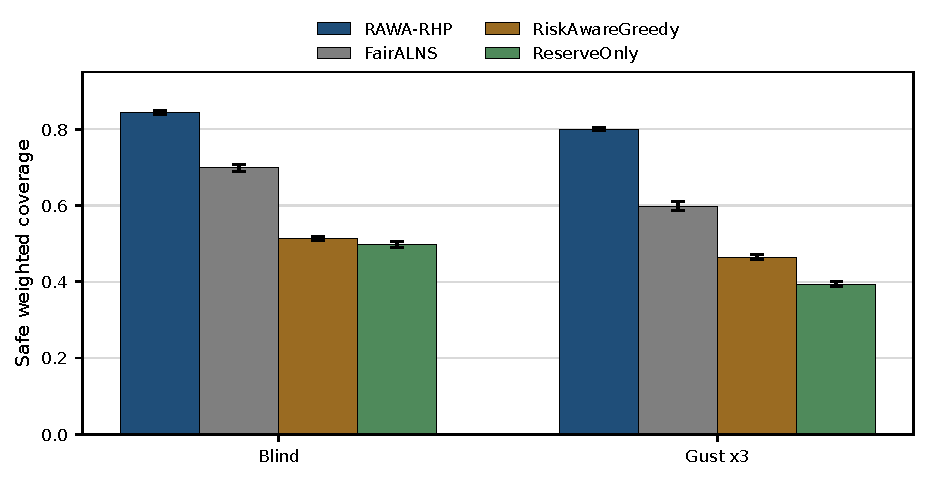
\includegraphics[width=0.82\textwidth]{figures/baseline_comparison.pdf}
    \caption{Safe weighted coverage in blind and gust-stress scenarios. Bars show means over paired episodes with SE error bars; paired 95\% confidence intervals are reported in Table~\ref{tab:baseline-stats}.}
    \label{fig:baseline}
\end{figure}

\begin{sloppypar}
The paired statistical comparison confirmed positive gains over FairALNS\-Planner, the strongest implemented baseline, under both scenario families (Table~\ref{tab:baseline-stats}). In blind scenarios, the paired SWC gain was 0.1447 with a 95\% confidence interval of [0.1307, 0.1591]. Under gust multiplier 3.0, the paired SWC gain was 0.2019 with a 95\% confidence interval of [0.1819, 0.2231]. Both comparisons were Holm-corrected significant, and the evaluated simulation hard-failure check rates were not worse.
\end{sloppypar}

\begin{table}[!htbp]
\centering
\caption{Paired statistical comparison against the strongest implemented baseline. The statistical unit is the scenario seed; confidence intervals use 10000 seed-clustered bootstrap resamples and Holm correction is applied within each reported comparison family.}
\label{tab:baseline-stats}
\resizebox{\textwidth}{!}{%
\begin{tabular}{llccccc}
\hline
Scenario & Strongest implemented baseline & Pairs & Mean diff. & 95\% CI & Holm $p$ & Simulation checks not worse \\
\hline
Blind & FairALNSPlanner & 600 & 0.1447 & [0.1307, 0.1591] & 0.00015 & Yes \\
Gust $\times 3$ & FairALNSPlanner & 400 & 0.2019 & [0.1819, 0.2231] & 0.00015 & Yes \\
\hline
\end{tabular}
}
\end{table}


\FloatBarrier

\subsection{Fixed-pipeline components remain positive under equal-budget ablations}

The fixed RAWA-RHP pipeline depended on all five retained components under native and equal-budget protocols. Removing RR-CMP caused the largest paired SWC loss: 0.1640 in Native and EqTime, and 0.1446 in EqEval (Table~\ref{tab:ablation} and Figure~\ref{fig:ablation}). Within this fixed pipeline, RR-CMP was the main source of additional coverage after a route had passed the return, reserve and clearance checks.

\begin{table}[!htbp]
\centering
\caption{Formal full-mode ablation results. Mean difference is RAWA-RHP minus the ablated planner in safe weighted coverage. Each row uses 360 paired scenarios; confidence intervals use seed-clustered bootstrap resampling.}
\label{tab:ablation}
\resizebox{\textwidth}{!}{%
\begin{tabular}{llccccc}
\hline
Module & Protocol & Episodes & Mean diff. & 95\% CI & Holm $p$ & Budget check \\
\hline
NoPacking & Native & 720 & 0.1640 & [0.1588, 0.1690] & 0.00075 & n/a \\
NoPacking & EqTime & 720 & 0.1640 & [0.1589, 0.1690] & 0.00075 & pass \\
NoPacking & EqEval & 720 & 0.1446 & [0.1391, 0.1499] & 0.00075 & pass \\
NoAdaptiveSearch & Native & 720 & 0.0462 & [0.0416, 0.0510] & 0.00075 & n/a \\
NoAdaptiveSearch & EqTime & 720 & 0.0462 & [0.0415, 0.0510] & 0.00075 & pass \\
NoAdaptiveSearch & EqEval & 720 & 0.0282 & [0.0243, 0.0317] & 0.00075 & pass \\
BlindReserve & Native & 720 & 0.0411 & [0.0390, 0.0431] & 0.00075 & n/a \\
BlindReserve & EqTime & 720 & 0.0411 & [0.0390, 0.0431] & 0.00075 & pass \\
BlindReserve & EqEval & 720 & 0.0418 & [0.0392, 0.0443] & 0.00075 & pass \\
NoRisk & Native & 720 & 0.0335 & [0.0311, 0.0357] & 0.00075 & n/a \\
NoRisk & EqTime & 720 & 0.0336 & [0.0313, 0.0357] & 0.00075 & pass \\
NoRisk & EqEval & 720 & 0.0331 & [0.0307, 0.0354] & 0.00075 & pass \\
NoBeam & Native & 720 & 0.0181 & [0.0142, 0.0222] & 0.00075 & n/a \\
NoBeam & EqTime & 720 & 0.0181 & [0.0142, 0.0222] & 0.00075 & pass \\
NoBeam & EqEval & 720 & 0.0171 & [0.0135, 0.0208] & 0.00075 & pass \\
\hline
\end{tabular}
}
\end{table}


\begin{figure}[t]
    \centering
    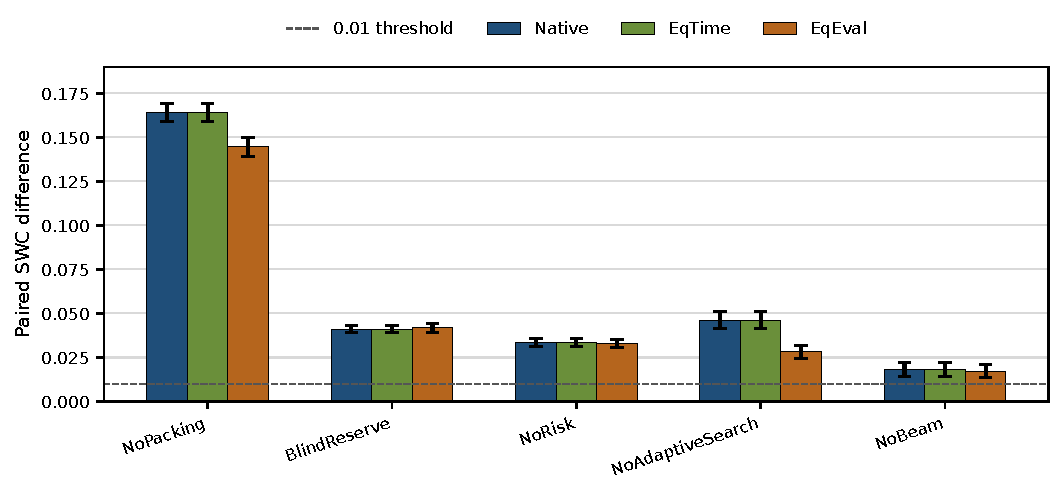
\includegraphics[width=0.86\textwidth]{figures/ablation_contributions.pdf}
    \caption{Core ablation contributions under native, equal-time and equal-evaluation protocols. Bars show paired mean differences with 95\% confidence intervals; budget-pass indicators are reported in Table~\ref{tab:ablation}.}
    \label{fig:ablation}
\end{figure}

The remaining ablations were smaller but stayed positive. NoAdaptiveSearch produced a 0.0462 loss under Native and EqTime and a 0.0282 loss under EqEval. BlindReserve produced a loss of about 0.041 across protocols, showing that reserve adaptation contributed within the fixed pipeline even when risk scoring remained active. NoRisk produced a loss of about 0.033, and NoBeam produced a smaller loss of about 0.017--0.018. These effects show useful pipeline dependencies, not that the mature components are individually new.

The EqEval checks met the required 5\% tolerance for all reported variants. The unified evaluation ratios ranged from 0.9538 to 0.9995 (Table~\ref{tab:eqeval-budget}), so the equal-evaluation results do not attribute the ablation gains to evaluating substantially more candidates.

\begin{table}[!htbp]
\centering
\caption{EqEval budget matching based on unified evaluation count.}
\label{tab:eqeval-budget}
\begin{tabular}{lc}
\hline
Variant & Unified evaluation ratio \\
\hline
RAWA-NoPacking-EqEval & 0.9995 \\
RAWA-NoBeam-EqEval & 0.9707 \\
RAWA-NoRisk-EqEval & 0.9538 \\
RAWA-BlindReserve-EqEval & 0.9754 \\
RAWA-NoAdaptiveSearch-EqEval & 0.9818 \\
\hline
\end{tabular}
\end{table}


\FloatBarrier

\subsection{Simulation hard-failure checks and latency meet benchmark gates}

RAWA-RHP was hard-failure-free in the proposed benchmark under the evaluated formal full-mode simulation checks. It had zero battery violations, zero clearance violations, zero reserve shortfalls, zero return failures and zero emergency aborts in that check. In the strict latency benchmark, which used a single worker, a fixed core, warm-up and identical trajectory inputs, RAWA-RHP produced 9962 replan samples over 360 episodes. Timing covers planner replanning, candidate expansion, risk queries and wind-energy budget queries from the precomputed edge cache; edge-cache construction and simulator execution are excluded. The p50, p95 and p99 replan latencies were 0.3314 s, 1.7549 s and 1.7590 s, respectively, with a maximum of 1.7917 s and a deadline miss rate of zero (Table~\ref{tab:latency} and Figure~\ref{fig:latency}). The closeness of p95 and p99 reflects the fixed 1.75 s replan budget, which concentrates high-quantile latency near the budget boundary.

\begin{table}[!htbp]
\centering
\caption{Strict latency benchmark under single-worker, fixed-core execution. Timing covers planner replanning, candidate expansion, risk and wind-energy budget queries from the precomputed edge cache; edge-cache construction and simulator execution are excluded.}
\label{tab:latency}
\resizebox{\textwidth}{!}{%
\begin{tabular}{ll}
\hline
Metric & Value \\
\hline
Hardware & Intel Core i9-9980XE CPU @ 3.00 GHz; Ubuntu Linux 6.8 \\
Language/runtime & Python 3.10.19 \\
Execution mode & single worker; fixed core; warm-up before measurement \\
Collision/wind-field timing scope & includes cached clearance-risk and wind-energy budget lookups; excludes edge-cache construction \\
Episodes & 360 \\
Replan samples & 9962 \\
p50 & 0.3314 s \\
p95 & 1.7549 s \\
p99 & 1.7590 s \\
Max & 1.7917 s \\
Deadline miss rate & 0.0000 \\
Hard failures in simulation checks & 0 \\
\hline
\end{tabular}
}
\end{table}


\begin{figure}[t]
    \centering
    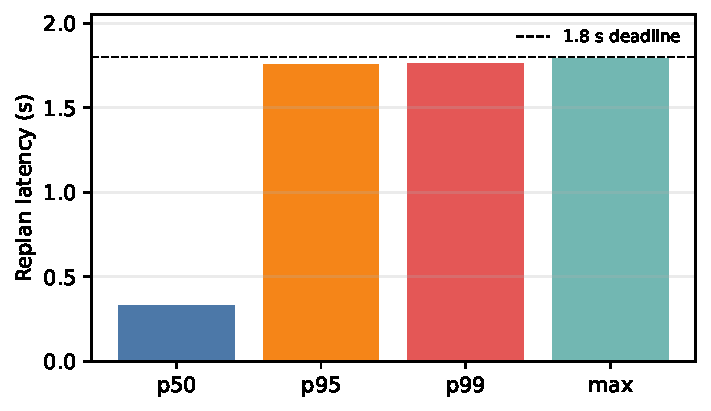
\includegraphics[width=0.68\textwidth]{figures/latency_benchmark.pdf}
    \caption{Strict replan latency benchmark. RAWA-RHP meets the 1.8 s p95 deadline and stays below the 2.2 s p99 requirement; edge-cache construction and simulator execution are excluded.}
    \label{fig:latency}
\end{figure}

\FloatBarrier

\subsection{Sensitivity and model-validity checks bound the parameter claims}

The additional sensitivity subset supports the use of the fixed final configuration while showing which settings matter most. Across 126 paired scenarios and 2772 sensitivity episodes, all variants had zero battery violations, clearance violations, reserve shortfalls, return failures and emergency aborts. Changing q90 to q80 or q95 changed mean SWC by +0.0047 and +0.0037, respectively, and changing the reserve buffer from 16 to 8 or 24 changed mean SWC by +0.0033 and -0.0017. Horizon length, RR-CMP weight scaling, clearance threshold and replan cap changes mostly stayed within about 0.005 mean SWC of the final setting. The largest changes came from reserve floor and search budget: reserve floor 60 increased mean SWC by 0.0127, reserve floor 100 reduced it by 0.0119, and halving the beam/search budget reduced mean SWC by 0.0239. These results indicate a reasonably broad plateau around the final configuration, with reserve conservatism and search budget as the main calibration-sensitive choices.

The model-validity checks were also consistent with the intended planning-layer abstraction. The energy curves were non-negative and responded monotonically to adverse wind components, while the clearance-risk curves decreased with clearance margin and increased under stronger crosswind/gust dispersion. These checks support bounded simulation plausibility only; they do not validate real-world flight energy, collision probability or low-level avoidance behaviour.

\section{Discussion}

\subsection{Why the selected application scenario fits RAWA-RHP}

The experiments suggest that RAWA-RHP is best matched to infrastructure inspection tasks where wind, clutter and return reserve are all active constraints. This includes coastal and mountainous transmission lines, wind farms, bridge structures and narrow corridor-like assets. These environments amplify the value of coupling reward search with return feasibility, but that coupling alone is not the main novelty. Wind-aware q90 energy estimates, adaptive reserve, clearance-risk control and beam search are mature planning ingredients. The main algorithmic role of RAWA-RHP is to make those checks define a residual feasible margin, then let RR-CMP convert part of that margin into additional inspection coverage.

The same setting also reduces the practical cost of the algorithm's main weakness. RAWA-RHP costs more computation than simple greedy planners, and in easy open-area missions its coverage advantage can be smaller. Infrastructure inspection, however, is commonly planned at a seconds-level decision cadence rather than as a millisecond-level inner-loop collision-avoidance controller. The strict latency benchmark showed that RAWA-RHP met the p95 and p99 replanning limits in this evaluated regime.

\subsection{Interpreting the ablations}

The largest fixed-pipeline dependency came from RR-CMP. This is consistent with the mission structure: inspection tasks often have spare fragments of energy or time that are too small for a full greedy detour but large enough for a carefully inserted target. This is the clearest algorithmic contribution in the paper. It reframes post-processing as residual-margin use rather than unconstrained route improvement.

Risk and reserve components also showed stable contributions. The BlindReserve and NoRisk ablations separate two effects: scoring risk and adapting reserve to risk. Both were useful within the evaluated pipeline, but this should be interpreted as an engineering dependency rather than a claim that risk-aware or reserve-aware UAV planning is new. The relevant finding is that RR-CMP benefits from having those feasibility margins available before packing.

Adaptive search remained positive even under EqEval, where the total evaluation count was matched. This indicates that the benefit comes from allocation of effort, not only from more effort. NoBeam had the smallest effect, but it remained significant, suggesting that retaining multiple route prefixes helps avoid local choices even when most of the gain is delivered by packing and reserve-aware risk control.

\subsection{What RAWA-RHP is not}

RAWA-RHP is not a new planning paradigm, a full stochastic optimal-control solver, a low-level collision-avoidance controller or hardware flight validation. It uses q90 budgets, reserve rules, risk filtering and beam search as established components inside a repeated planning loop. It should sit above a controller that handles vehicle dynamics, tracking and immediate obstacle avoidance. The method also is not necessary for easy open-area low-wind surveys where a simpler planner may be sufficient; its intended use is the harder case where wind, clutter and return reserve make coverage-only routing unreliable.

\subsection{Limitations}

The study is simulation-based. Although the scenarios include wind levels, correlated gusts, narrow passages and obstacle-density variation, they do not replace hardware flight tests around real infrastructure. The energy and risk models are abstractions; performance depends on the calibration quality of the wind-energy and clearance-risk models. The sensitivity subset shows that reserve conservatism and search budget affect SWC, so these settings should be recalibrated before transferring the planner to another simulator or vehicle envelope. RAWA-RHP is not intended as a millisecond-level collision-avoidance controller. It should be used above a low-level controller that handles vehicle dynamics and immediate obstacle avoidance.

Another limitation is that the method is designed for missions where evaluated return, reserve and clearance-risk constraints interact with coverage. In low-wind, open, low-risk surveys, a simpler planner may be easier to deploy and may offer sufficient performance. The main claim of this paper is therefore bounded: RAWA-RHP is most appropriate for wind-affected inspection routing where losing return reserve or clearance margin is central to the benchmark objective.

\section{Conclusion}

The paired comparison showed that RAWA-RHP improved SWC over the strongest implemented baseline by 0.1447 in blind scenarios and 0.2019 under gust stress, with positive 95\% confidence intervals and Holm-corrected significance. The formal ablation study identified RR-CMP as the largest fixed-pipeline dependency and showed smaller positive dependencies for adaptive search, risk control, adaptive reserve and beam search under native, equal-time and equal-evaluation protocols. The strict latency benchmark showed p95/p99 replanning latencies of 1.7549/1.7590 s and zero hard failures in the evaluated formal simulation checks. Together, these results provide bounded planning-layer simulation evidence for residual-margin packing in wind-affected infrastructure inspection.

\section*{Declaration of competing interest}
The authors declare no competing interests.

\section*{Data availability}
The data and code reproduction package for this study is available at\url{https://github.com/lhaochen419-del/rawa-rhp-reproduction} and archivedat \url{https://doi.org/10.5281/zenodo.21200028}. The package containsscenario definitions and seeds, planner configuration files, episode-levelraw simulation outputs, processed result tables, figure source data, latencysamples, statistical analysis outputs, parameter-sensitivity outputs,simulation-model validity-check source data and scripts needed to regeneratethe reported tables and figures. The source code includes the simulator,RAWA-RHP implementation, implemented baseline planners, analysis scripts,plotting scripts and environment specification. A verification scriptreproduces the main paired baseline differences, ablation summaries andlatency statistics reported in the manuscript.

\section*{Funding}
\begin{itemize}
\item Macao Polytechnic University (MPU Grant no. RP/FCA-01/2025).
\item \begin{sloppypar}Macao Science and Technology Development Fund (FDCT-MOST:\allowbreak{} 0018/\allowbreak{}2025/\allowbreak{}AMJ).\end{sloppypar}
\end{itemize}

\section*{CRediT authorship contribution statement}
H.L. conceived and designed the study. H.L. and J.W. developed the methodology and implemented the software. H.L., J.W., D.Y., Y.Z. and Y.L. performed the validation and formal analysis. Z.M., J.Y., H.L. and J.W. carried out the investigation. D.Y., S.-K.I., Y.W. and X.Y. provided the resources. Z.M., J.Y. and B.L. performed the data curation. Z.M., J.Y., H.L. and J.W. prepared the original draft. H.L., J.W., D.Y., S.-K.I., Y.W. and X.Y. reviewed and edited the manuscript. H.L., Y.Z., Y.L. and D.Y. contributed to the visualization. D.Y., S.-K.I., Y.W. and X.Y. supervised the research and managed the project. D.Y., S.-K.I., Y.W. and X.Y. acquired the funding. All authors reviewed the manuscript.

\section*{Acknowledgements}
\begin{sloppypar}
Support from Macao Polytechnic University (RP/FCA-01/2025) and the Macao Science and Technology Development Fund (FDCT-MOST:\allowbreak{} 0018/\allowbreak{}2025/\allowbreak{}AMJ) enabled data collection, analysis and interpretation, and covered research materials and computational experiments. MPU and FDCT investment in our work significantly contributed to the quality and impact of our research findings.
\end{sloppypar}

\bibliographystyle{elsarticle-num-names}
\bibliography{references}

\end{document}
